\chapter{实验环境搭建}

\section{仿真环境配置}

\subsection{Carla 仿真平台}


CARLA 是一个开源的自动驾驶仿真平台,可提供超高真实度的交通环境,车辆动力学模型。在这个项目中,我们选择使用 CARLA 的 Town10 模拟场景进行试验, Town10 场景具有多处十字路口、不同种类的车道以及大量的交通元素,能够模拟实际交通中的各种复杂环境,是研究多目标跟踪算法理想的起点。

版本选择:本次设计中安装的是Carla0.9.15版本,该版本的功能以及稳定性完全可以满足我们的实验需求。

地图导入:从Carla的客户端程序导入Town10地图,要保证地图中的道路、房屋、路标等都成功导入。
传感器设置:为车辆在 Carla 中安装多种类型的传感器,例如 RGB 摄像头、深度摄像头和雷达。其中 RGB 摄像头是用来拍摄交通环境的视觉图片,深度摄像头与雷达用来测量物体之间的距离,传感器收集的信息将提供给多目标跟踪算法。按照试验要求合理调整设定传感器的参数,分辨率、帧率、视野等,以便获取高精度的仿真数据。



\subsection{Pycharm环境配置}

依据课题需求,本项目还进一步构建了基于 Town10 仿真实景的交通数字孪生系统,以进行获取目标真值轨迹(Grouth Truth)以及检 测跟踪模型优化。

环境构建:首先,依据项目及课题需求,构建 Python 3.8 虚拟环境,安装类似表 4-1 中的核心依赖包。

航点控制与轨迹插值:使用该项目航点控制模块得到车在 Town10 环境下的运行航点。采用轨迹插值算法生成连续路径,主要运用scipy信号处理库及numpy数值运算,所用相关算法实现方式见表~\ref{tab:full-dependencies}科学计算库。

PID控制器:通过PID控制算法对小车进行控制,主要的实现使用numpy来进行矩阵计算,并且用matplotlib来实现控制过程可视化。实时数据显示工具dash在表~\ref{tab:full-dependencies}中用来实现控制参数调节界面。


\begin{table}[htbp]
	\centering
	\caption{Python 虚拟环境完整依赖清单}
	\label{tab:full-dependencies}
	\begin{tabular}{lll}
		\hline
		\textbf{类别} & \textbf{包名称} & \textbf{版本} \\ 
		\hline
		\multirow{8}{*}{核心依赖}
		& numpy & 1.24.4 \\
		& scipy & 1.10.1 \\
		& protobuf & $\geq$3.6 \\
		& future & $\geq$0.16.0 \\
		& psutil & 6.1.0 \\
		& opencv-python & 4.10.0.84 \\
		& pillow & 10.4.0 \\
		& open3d & 0.18.0 \\
		
		\hline
		\multirow{6}{*}{仿真交互}
		& carla & 0.9.15 \\
		& pygame & $\geq$1.9.4 \\
		& pywin32 & 308 \\
		& configargparse & 1.7 \\
		& retrying & 1.3.4 \\
		& tenacity & 9.0.0 \\
		
		\hline
		\multirow{7}{*}{数据处理}
		& pandas & 2.0.3 \\
		& python-dateutil & 2.9.0.post0 \\
		& pyparsing & 3.1.4 \\
		& contourpy & 1.1.1 \\
		& cycler & 0.12.1 \\
		& fonttools & 4.55.1 \\
		& packaging & 24.2 \\
		
		\hline
		\multirow{6}{*}{可视化}
		& matplotlib & 3.7.5 \\
		& plotly & 5.24.1 \\
		& dash & 2.18.2 \\
		& dash-core-components & 2.0.0 \\
		& dash-html-components & 2.0.0 \\
		& dash-table & 5.0.0 \\
		
		\hline
		\multirow{8}{*}{开发工具}
		& ipython & 8.12.3 \\
		& jedi & 0.19.2 \\
		& traitlets & 5.14.3 \\
		& prompt-toolkit & 3.0.48 \\
		& pygments & 2.18.0 \\
		& wcwidth & 0.2.13 \\
		& platformdirs & 4.3.6 \\
		& executing & 2.1.0 \\
		
		\hline
		\multirow{6}{*}{Web框架}
		& flask & 3.0.3 \\
		& werkzeug & 3.0.6 \\
		& jinja2 & 3.1.5 \\
		& itsdangerous & 2.2.0 \\
		& click & 8.1.8 \\
		& blinker & 1.8.2 \\
		
		
		
		\hline
	\end{tabular}
\end{table}


\subsection{Matlab环境配置}

版本:Matlab2024b,如图\ref{fig:p7}matlab环境。


\begin{figure}[htbp] % 可以是h(here),t(top),b(bottom),p(page of floats)
	\centering
	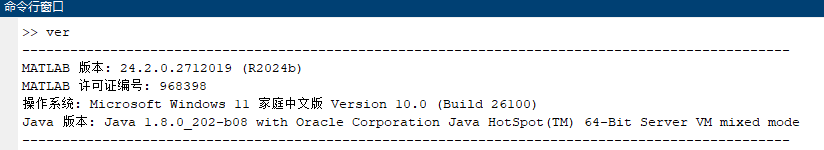
\includegraphics[width=1\textwidth]{p7} % 假设图片文件名为car.pdf或car.png等,位于当前工作目录
	\caption{matlab环境} % 图片标题
	\label{fig:p7} % 用于引用的标签
\end{figure}


MATLAB 算法开发平台,它的 image processing toolbox 和 computer vision toolbox 为多目标跟踪算法的开发提供各种强大的工具及函数。使用这些工具箱,可以迅速将各种多目标跟踪算法实现出来进行测试,比如卡尔曼滤波、联合概率数据关联滤波这些经典算法,以及结合深度学习的目标检测和跟踪算法。将这些算法在 MATLAB 中实现以后,会比较容易对算法进行测试,调试,然后与目前的Baseline算法进行对比研究。


而在实验中采集的数据又是那么多那么杂,但好在MATLAB数据处理工具箱非常强大,例如:信号处理工具箱、统计和机器学习工具箱如图\ref{fig:p8}所示能够快速有效的对交通环境下的传感器的数据预处理,特征点提取以及统计。例如,可以利用这些工具箱过 滤并删除从Carla仿真平台上采集的车辆轨迹中的噪声,并从中提取有效信息关键点以及对于多目标的运动模型进行构建分析。




\begin{figure}[htbp] % 可以是h(here),t(top),b(bottom),p(page of floats)
	\centering
	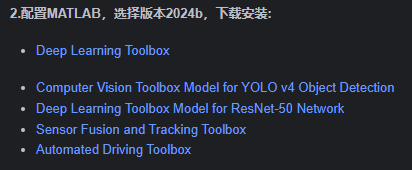
\includegraphics[width=1\textwidth]{p8} % 假设图片文件名为car.pdf或car.png等,位于当前工作目录
	\caption{matlab配置} % 图片标题
	\label{fig:p8} % 用于引用的标签
\end{figure}






\section{实验设备与软件工具}

\subsection{硬件设备}

设备名称:DESKTOP-H2JCRHP

处理器:AMD Ryzen 7 5800H with Radeon Graphics            3.20 GHz

机带:RAM	16.0 GB (15.4 GB 可用)

设备 ID:9FF8ABE5-216E-4C15-B738-D4364271428F

产品 ID:00326-40000-00000-AAOEM

系统类型:64 位操作系统, 基于 x64 的处理器

GPU:NVIDlA GeForce RTX 3060 Laptop GPU 与 Radeon(TM) Graphics

内存:1.32TB

此硬件可使 Carla 模拟器启动运行,并确保多目标跟踪算法的快速训练与测试。另加装了大容量固态硬盘(SSD),可以存储 Carla的场景与传感器数据,以及实验过程中产生的大量模型与结果数据,能够实现快速的数据读取与写入,并保证数据安全。

\subsection{软件工具}

拥有全面的软件工具才能让设计顺利地进行,如图\ref{fig:p31}是本次设计所需要的软件工具。

操作系统:Windows 11

本研究的编程语言主要选 Python,用它来开发算法和写实验脚本。开发工具是 PyCharm,它集成了代码编辑、调试、版本控制等功能,方便又高效。另外,装好了 carla、NumPy、SciPy、OpenCV 等常用 Python 库,这些库在数据处理、图像处理和数学计算方面都很好用。

深度学习框架选的是 PyTorch,这框架模型构建灵活,还有强大的自动微分功能,特别适合实现和优化多目标跟踪模型。同时,安装了 torchvision 等相关依赖包,为模型的训练和测试提供了坚实的支持。
数据库管理系统用的是 MySQL,用它搭建了路口车辆航点到 Carla 坐标映射的数据库。创建了相应的数据表,存储路口、车道、方向等信息以及对应的 Carla 场景中道路终点坐标位置(x, y, z 和 yaw),为路口导航和目标跟踪提供了可靠的数据支持。

数据预处理和格式转换这块,本此设计选择的是Matlab2024b 工具。它能做多模态数据处理、快速验证算法和量化评估性能,还配备了 Computer Vision Toolbox、Sensor Fusion and Tracking Toolbox 等丰富的工具箱,大大提高了开发效率。在轨迹优化、跨传感器融合和可视化方面,它提供了高效的解决方案,对智慧交通场景下多目标跟踪算法的研究和实际应用都有很大的帮助。




备有完备的软件工具才能使设计顺利展开。如下图\ref{fig:p31}为此次设计所需用的软件工具。

操作系统:Windows 11

本课题程序语言主要是 Python 语言,用于编写算法以及实验脚本。使用开发工具有 Pycharm,包含代码编写、调试、版本管理等功能,简洁方便。同时安装了常用的python库如carla、NumPy、SciPy、OpenCV,这些库对于数据处理、图像处理与数学运算都很友好。

深度学习框架采用 Pytorch,该框架模型构建自由,具有强大的自动微分功能非常适合对多目标跟踪模型进行实现及优化。同时安装 torchvision 等一系列依赖库,使得模型的训练及测试能够顺利进行。数据库管理系统采用 MySQL,使用 MySQL 构建了路口车辆航点到 Carla场景坐标映射的数据库。建立了相应的表,存储路口,车道,方向等一系列信息及对应 Carla 场景中的道路终点坐标位置(x, y, z, yaw),为路口导航和目标跟踪提供数据支持。

数据的预处理及格式转换。本次的设计选用了Matlab2024b进行。它可以进行多种模式的数据处理,可以快速地测试算法并对性能进行量化的评估,而且拥有Computer Vision Toolbox Sensor Fusion and Tracking Toolbox等众多的工具箱,开发效率非常高。在航迹优化、跨传感器融合以及可视化上都带来了高效的方案,对于智能交通环境下的多目标追踪算法的研究与应用都有非常大的帮助。



\begin{figure}[htbp] % 可以是h(here),t(top),b(bottom),p(page of floats)
	\centering
	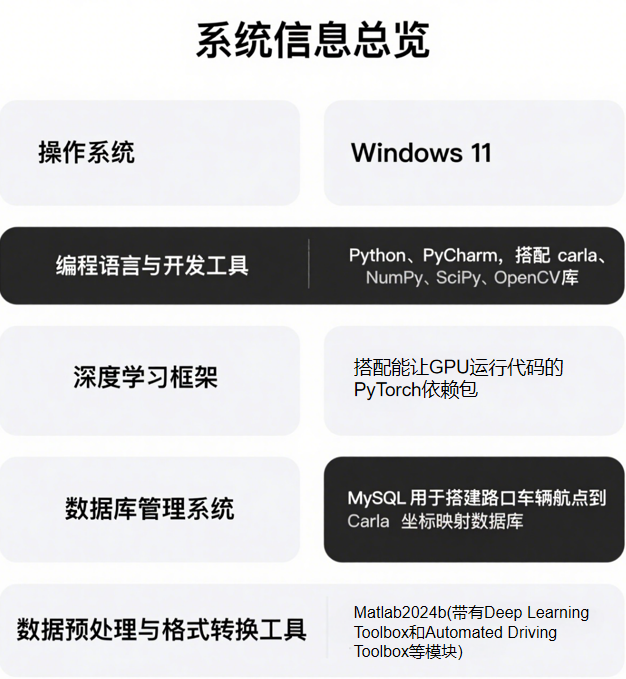
\includegraphics[width=0.75\textwidth]{p31} % 假设图片文件名为car.pdf或car.png等,位于当前工作目录
	\caption{软件工具} % 图片标题
	\label{fig:p31} % 用于引用的标签
\end{figure}









